\section{Arquitectura}

\begin{itemize}

    \item{Descripción General}

MindWave es un sistema avanzado diseñado para la adquisición y procesamiento de señales electroencefalográficas (EEG), con un diseño modular y escalable. Este sistema consta de varios módulos interconectados que aseguran una alta precisión en la captura de datos, estabilidad durante el proceso de adquisición y flexibilidad para su aplicación en investigación y diagnóstico clínico. Los electrodos, posicionados según el sistema 10-20, capturan señales eléctricas del cerebro y las transmiten a un módulo de conversión analógica a digital. Posteriormente, estas señales digitalizadas son gestionadas por un microcontrolador, que no solo regula el flujo de datos, sino que también monitorea la calidad de las señales adquiridas. Finalmente, el sistema se conecta a una plataforma de software que permite la visualización en tiempo real, el almacenamiento seguro de datos en servicios en la nube y la sincronización precisa con los eventos experimentales, facilitando así el análisis posterior, como se muestra en la figura \ref{fig:Esquema}.

\begin{figure}
    \centering
    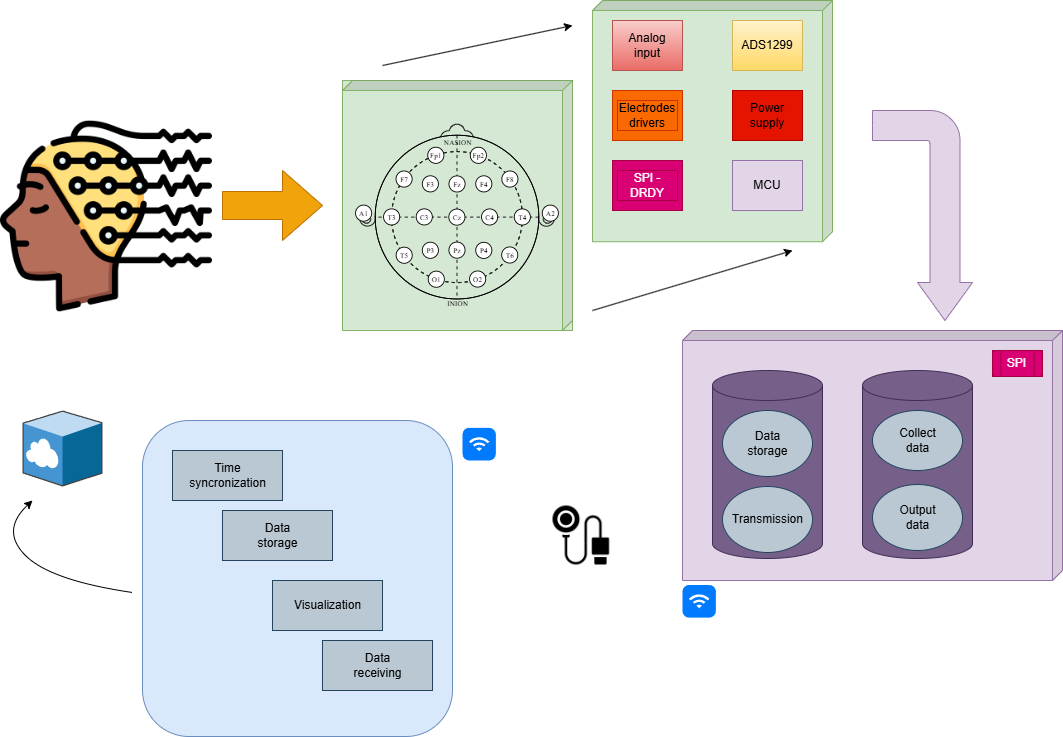
\includegraphics[width=0.8\linewidth]{Figures/DBP.png}
    \caption{Arquitectura de MindWave}
    \label{fig:Esquema}
\end{figure}

    \item {Módulo de Transmisión}

El módulo de transmisión de MindWave sirve como el centro neurálgico que conecta la adquisición de señales con su procesamiento y visualización externa. Consiste en varios subsistemas clave que operan de manera cohesionada:

    \item Módulo de Conversión Analógico-Digital

En el núcleo del módulo de adquisición se encuentra el ADS1299 de Texas Instruments \cite{TI_ADS1299}, un convertidor analógico-digital (ADC) de alta precisión diseñado específicamente para aplicaciones de monitoreo biológico como EEG, EMG y ECG. Este ADC presenta características que lo hacen ideal para capturar señales de baja amplitud, típicas de la actividad cerebral, como una resolución de 24 bits y un alto rango dinámico capaz de detectar variaciones sutiles en la actividad cerebral.

El ADS1299 incluye múltiples canales de entrada que pueden operar simultáneamente, lo que permite una adquisición de datos sincronizada. Además, tiene filtros digitales incorporados, como filtros pasa-bajo y notch, que ayudan a reducir el ruido y mejorar la relación señal-ruido antes de que las señales sean digitalizadas. Su capacidad para trabajar en configuraciones en cascada permite conectar hasta ocho módulos ADS1299, lo que soporta configuraciones de adquisición de datos de hasta 64 canales. Esto es esencial para estudios avanzados que requieren una cobertura amplia y detallada de la actividad cerebral.

    \item Transmisor

El sistema de transmisión de MindWave está diseñado para garantizar una transferencia rápida y confiable de los datos digitalizados a un dispositivo externo, como una computadora o servidor. Emplea un sistema de comunicación serial de alta velocidad, utilizando protocolos como UART o SPI, optimizados para minimizar la latencia durante la transmisión. Este enfoque asegura que los datos adquiridos puedan ser procesados o visualizados en tiempo real sin retrasos o pérdidas significativas, lo cual es crítico para aplicaciones que requieren una sincronización precisa, como experimentos en neurociencia o estudios clínicos con estimulación sincronizada.

Para asegurar conexiones eficientes y adaptables, el sistema puede integrar conversores USB-a-serial, lo que permite la compatibilidad con computadoras modernas sin interfaces seriales nativas. Además, MindWave puede incorporar transmisores inalámbricos, como módulos Bluetooth o Wi-Fi, para situaciones donde la movilidad o la eliminación de cables sea crucial. Sin embargo, la arquitectura inicial se centra en interfaces seriales por cable para priorizar la baja latencia y estabilidad.

    \item Microcontrolador

El microcontrolador elegido para MindWave debe manejar un alto volumen de datos provenientes de hasta 64 canales de EEG simultáneamente, además de supervisar los procesos de adquisición y comunicación. Una opción adecuada es el STM32H7 de STMicroelectronics \cite{STMicroelectronics_STM32H7}, basado en un núcleo ARM Cortex-M7. Este microcontrolador combina un rendimiento excepcional con una memoria RAM amplia y capacidades de procesamiento en tiempo real.

El STM32H7 incluye múltiples interfaces de comunicación, como SPI, I2C y UART, lo que permite la integración directa con los módulos ADS1299 y de transmisión. Su capacidad para manejar tareas paralelas asegura que pueda controlar múltiples módulos ADS1299 en configuraciones en cascada, gestionar la transmisión de datos a dispositivos externos y realizar operaciones de preprocesamiento básico, como detección de artefactos o validación de datos.

Además, su soporte para módulos de comunicación inalámbrica, incluyendo BLE y Wi-Fi, lo hace adaptable para futuras expansiones del sistema. Esto asegura que MindWave no solo cumpla con los requisitos actuales de adquisición, sino que también sea escalable para necesidades futuras.

    \item Software

La plataforma de software de MindWave está diseñada como una herramienta integral que proporciona visualización, almacenamiento y análisis de los datos de EEG. Esta plataforma, desarrollada con una interfaz gráfica amigable, permite a los investigadores y usuarios clínicos monitorear señales EEG en tiempo real con representaciones gráficas interactivas, incluyendo visualizaciones del espectro de frecuencias, tendencias temporales y patrones espaciales.

El software también se conecta a servicios de almacenamiento en la nube, lo que permite la copia de seguridad automática de los datos adquiridos y su accesibilidad para análisis remotos. Esta funcionalidad es esencial para proyectos colaborativos o investigadores que necesitan acceso a los datos desde diferentes ubicaciones geográficas.

Además de las características de visualización, la plataforma incluye un sistema de sincronización temporal que permite registrar eventos experimentales y asociarlos con las señales EEG correspondientes. Esto es particularmente útil en estudios que combinan estimulación visual o auditiva, ya que facilita la identificación de respuestas cerebrales específicas ante estímulos dados.

Las futuras implementaciones del software planean incluir herramientas de análisis automatizado basadas en inteligencia artificial, lo que permitirá a los investigadores identificar patrones complejos en los datos de EEG y generar informes detallados automáticamente.

\end{itemize}

